\section{Livello 2 Frame DHLC}


\subsection{Struttura del frame}
\begin{figure}[h!]
    \centering
    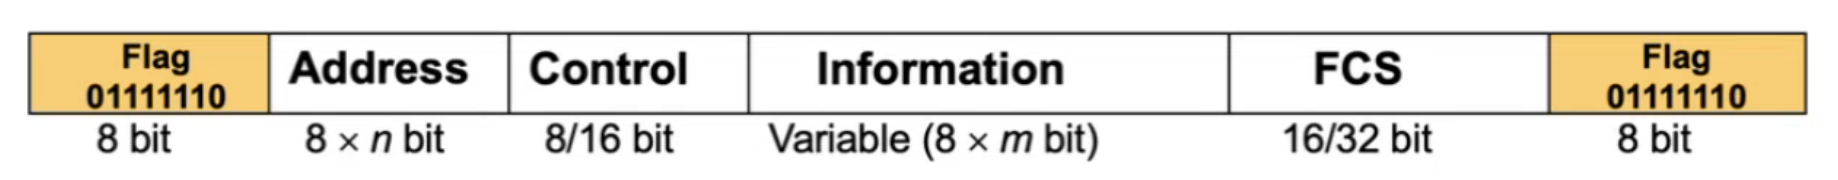
\includegraphics[width=0.8\textwidth]{images/strutturaframe.png}
    \caption{Struttura del frame HDLC}
    \label{fig:struttura-frame}
\end{figure}
\begin{itemize}
    \item flag: sono posti ad inizio e fine frame così da delimitare il frame e far capire a chi lo riceve quando inizia e quando finisce il frame, questi flag sono SEMPRE 8 bit in questa sequenza: 
01111110, ossia 7E in esadecimale
        \item address: indirizzo del trasmettitore, ricevitore o broadcast(se tutti 1)

    \begin{multicols}{2}
        \item control: indica il tipo di frame
        \item information: dati del livello superiore, payload
        \item FCS(frame check sequence): 
    \end{multicols}
\end{itemize}

\subsection{Bit stuffing}
 A proposito dei flag usati nel frame(011111110) che succede se questa sequenza invece fa parte della informazione utile del frame e non come flag delimitatore?

\begin{figure}[h!]
    \centering
    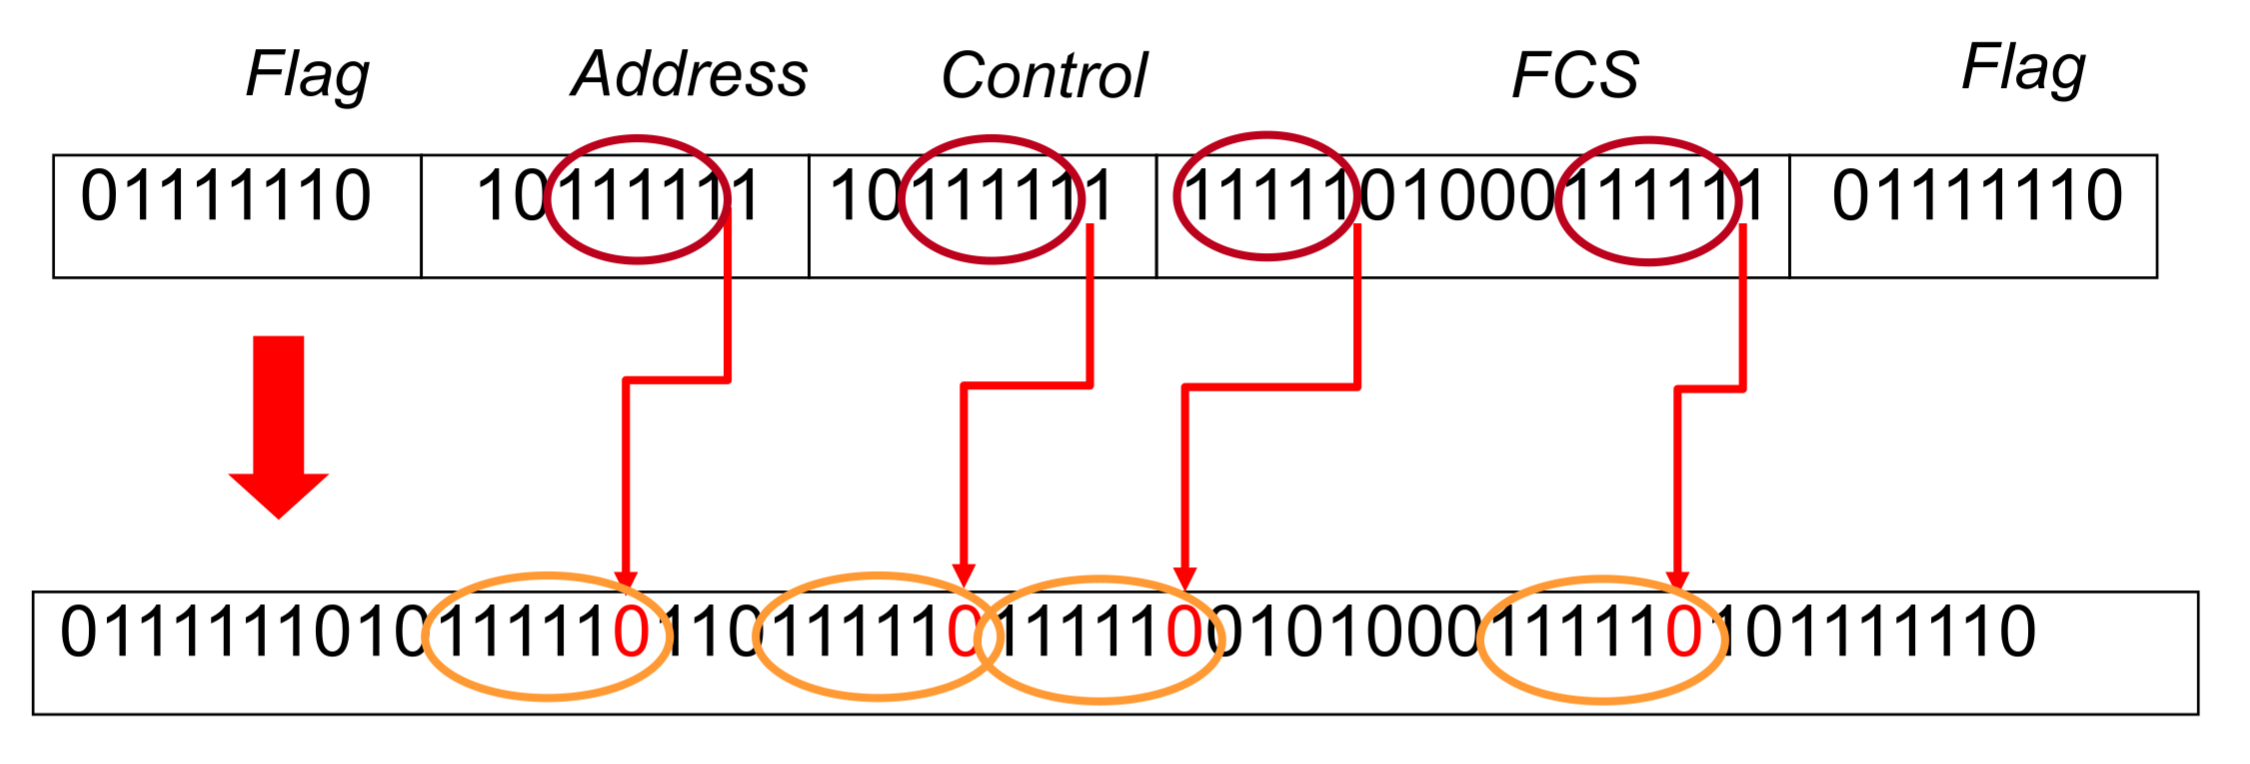
\includegraphics[width=0.8\textwidth]{images/bitstuffing.png}
    \caption{Esempio di bit stuffing}
    \label{fig:bit-stuffing}
\end{figure}
Risolvo inserendo uno 0 ogni cinque 1 ripetuti; questo fa perdere la molteplicità di 8 del frame.

\subsection{Rivelazione dell'errore con CRC}

HDLC numera i frame e usa il protocollo di linea, utilizzando 3 o 7 bit, usando una tecnica di piggybacking per gestire il flusso che viene dalla direzione opposta(finestre di trasmissione e ricezione).

Il CRC è un metodo per il calcolo di somme di controllo (checksum). Il nome deriva dal fatto che i dati d'uscita sono ottenuti elaborando i dati di ingresso i quali vengono fatti scorrere ciclicamente in una rete logica.

Sfrutta l'algebra dei campi finiti ed è utile per l'individuazione di errori casuali nella trasmissione dati (a causa di interferenze, rumore di linea, distorsione), il CRC non è invece affidabile per verificare la completa correttezza dei dati contro tentativi intenzionali di manomissione.
\paragraph{Polinomio generatore}
Un codice CRC è definito dal suo polinomio generatore di ordine r:

esempio r = 3

\begin{equation}
    G(x) = x^3 + x^2 + 1 \quad \Rightarrow \quad 1101
\end{equation}

\subsubsection{Cosa avviene in trasmissione}
 Con una scelta opportuna del polinomio generatore è possibile rilevare errori sul singolo bit etc... ;

 setup del CRC per la trasmissione:

\begin{figure}[htbp]
    \centering
    \begin{minipage}{0.45\textwidth}
        Traduco i bit che compongono header e payload in un polinomio P(x) di coefficienti d; perciò di grado d-1.
    \end{minipage}%
    \hfill
    \begin{minipage}{0.5\textwidth}
        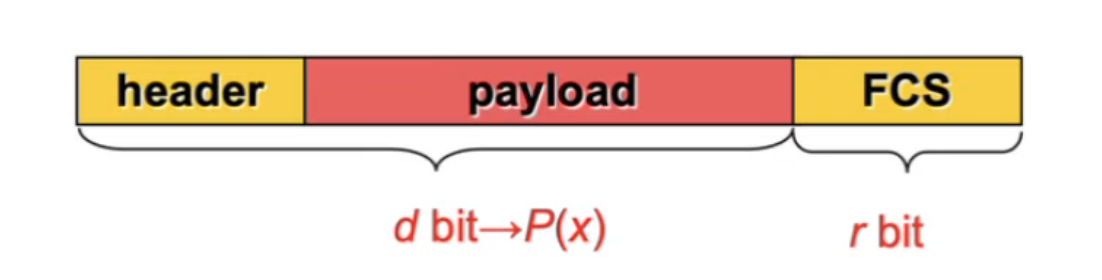
\includegraphics[width=\linewidth]{images/crctrasmissione.png}
        \caption{Schema del calcolo di CRC, P(x)}
    \end{minipage}
\end{figure}

\begin{figure}[htbp]
    \centering
   \begin{minipage}{0.5\textwidth}
        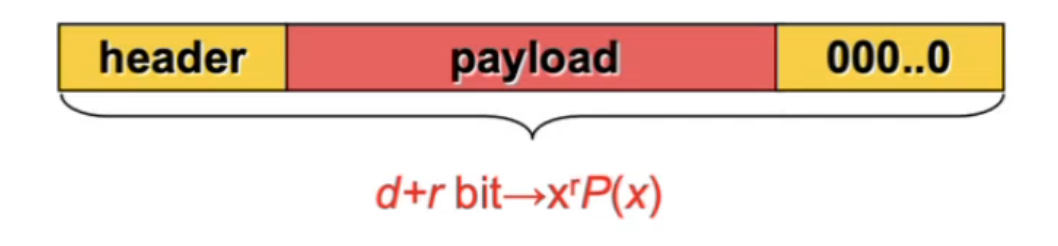
\includegraphics[width=\linewidth]{images/crcricezione.png}
        \caption{Schema del calcolo di CRC, $x^rP(x)$}
    \end{minipage}
    \hfill
     \begin{minipage}{0.45\textwidth}
        Si moltiplica P(x), ricavato qui sopra, per $x^r$(shift di r posizioni, le stesse del poliniomio generatore), ottendo il polinomio $x^rP(x)$ di grado d+r-1, con coefficienti d+r.
      
        In seguito allo shift, il campo FCS del frame sarà costutuito da r zeri.
    \end{minipage}%
\end{figure}

\paragraph{Calcolo e verifica del CRC in trasmissione}
In trasmissione si divide il polinomio $x^rP(x)$ per G(x), il resto di questa operazione[il polinomio R(x)] sono i bit del CRC, da inserire nel FCS del frame.
Vedi operatore XOR appendice basi.

\begin{equation}
    \frac{x^rP(x)}{G(x)} = Q(x) \oplus \frac{R(x)}{G(x)}
\end{equation}


\begin{figure}[htbp]
    \centering
    \begin{minipage}{0.45\textwidth}
        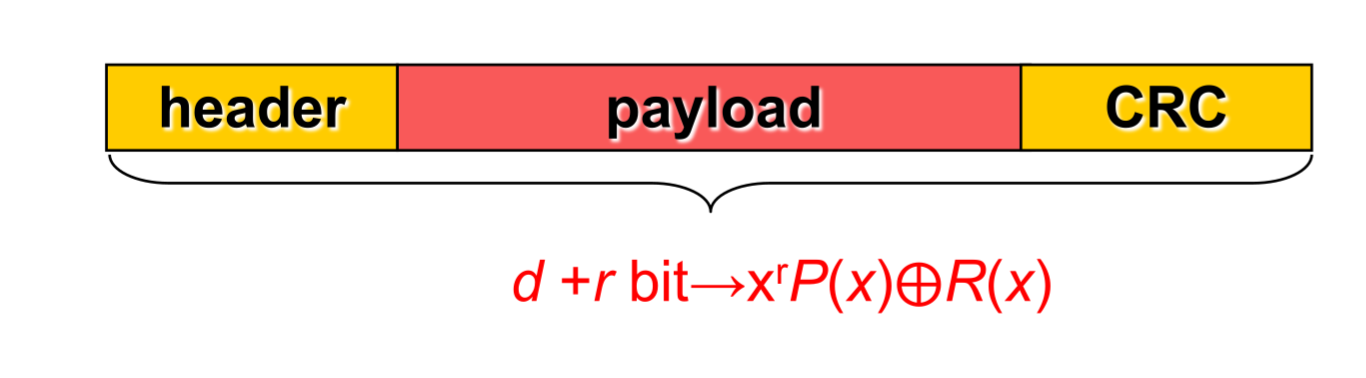
\includegraphics[width=\linewidth]{images/calcolocrc.png}
        \caption{Inserimento bit in FCS}
        \label{fig:calcolo-crc}
    \end{minipage}%
    \hfill
    \begin{minipage}{0.5\textwidth}
        Devo quindi inserire i bit del polonomio R(x) all'interno del FCS, effettuo l'operazione:
\begin{equation}
    P^{Tx} = x^rP(x) \oplus R(x)
\end{equation}
    \end{minipage}
\end{figure}
\newpage
\subsubsection{Verifica CRC}

C'è la necessità di verificare se il CRC calcolato ed inserito nel FCS sia corretto.
\paragraph{Polinomio relativo} è necessario calcolare il polonomio relativo $P^{Rx}(x)$ per verificare CRC; questo polinomio non è altro che la trama di d+r bit ricevuti in ricezione.
\paragraph{Condizione necessaria}
Infine per verificare CRC c'è da tenere a mente la condizione necessaria affinchè il CSC sia corretto, ossia che il resto della divisione tra polinomio relativo[$P^{Rx}(x)$] e polonomio generatore[G(x)] sia nullo:

\begin{equation}
    \frac{P^{Rx}(x)}{G(x)} = Q'(x) \oplus R'(x)
\end{equation}
Può accadere che il resto sia nullo con trama ricevuta errata (la condizione è necessaria, non sufficiente). 

Non si può quindi essere certi della correttezza della trama (c'è sempre una
probabilità non nulla di falso positivo).

Se il resto NON è nullo, invece, c'è la certezza che la trama sia errata
perché la condizione necessaria è stata violata

\paragraph{Dimostrazione condizione necessaria}
Nel caso in cui la trama ricevuta sia corretta, il polinomio che costruiamo da questa trama deve essere uguale al polinomio originale(trama trasmessa), cioè:
\begin{equation}
    P^{Rx}(x) = P^{Tx}(x)
\end{equation}

Se effettuiamo la divisione per il polinomio generatore:

    \begin{equation}
        \frac{P^{Rx}(x)}{G(x)} = \frac{P^{Tx}(x)}{G(x)} = \frac{x^rP(x) \oplus R(x)}{G(x)} = \frac{x^rP(x)}{G(x)} \oplus \frac{R(x)}{G(x)}
    \end{equation}
    \begin{equation}
        \frac{P^{Rx}(x)}{G(x)} = \frac{x^rP(x)}{G(x)} \oplus \frac{R(x)}{G(x)} = Q(x) \oplus \frac{R(x)}{G(x)} \oplus \frac{R(x)}{G(x)} = Q(x)
    \end{equation}

    \subsubsection{Esempio calcolo CRC}
    \begin{figure}[htbp]
        \centering
        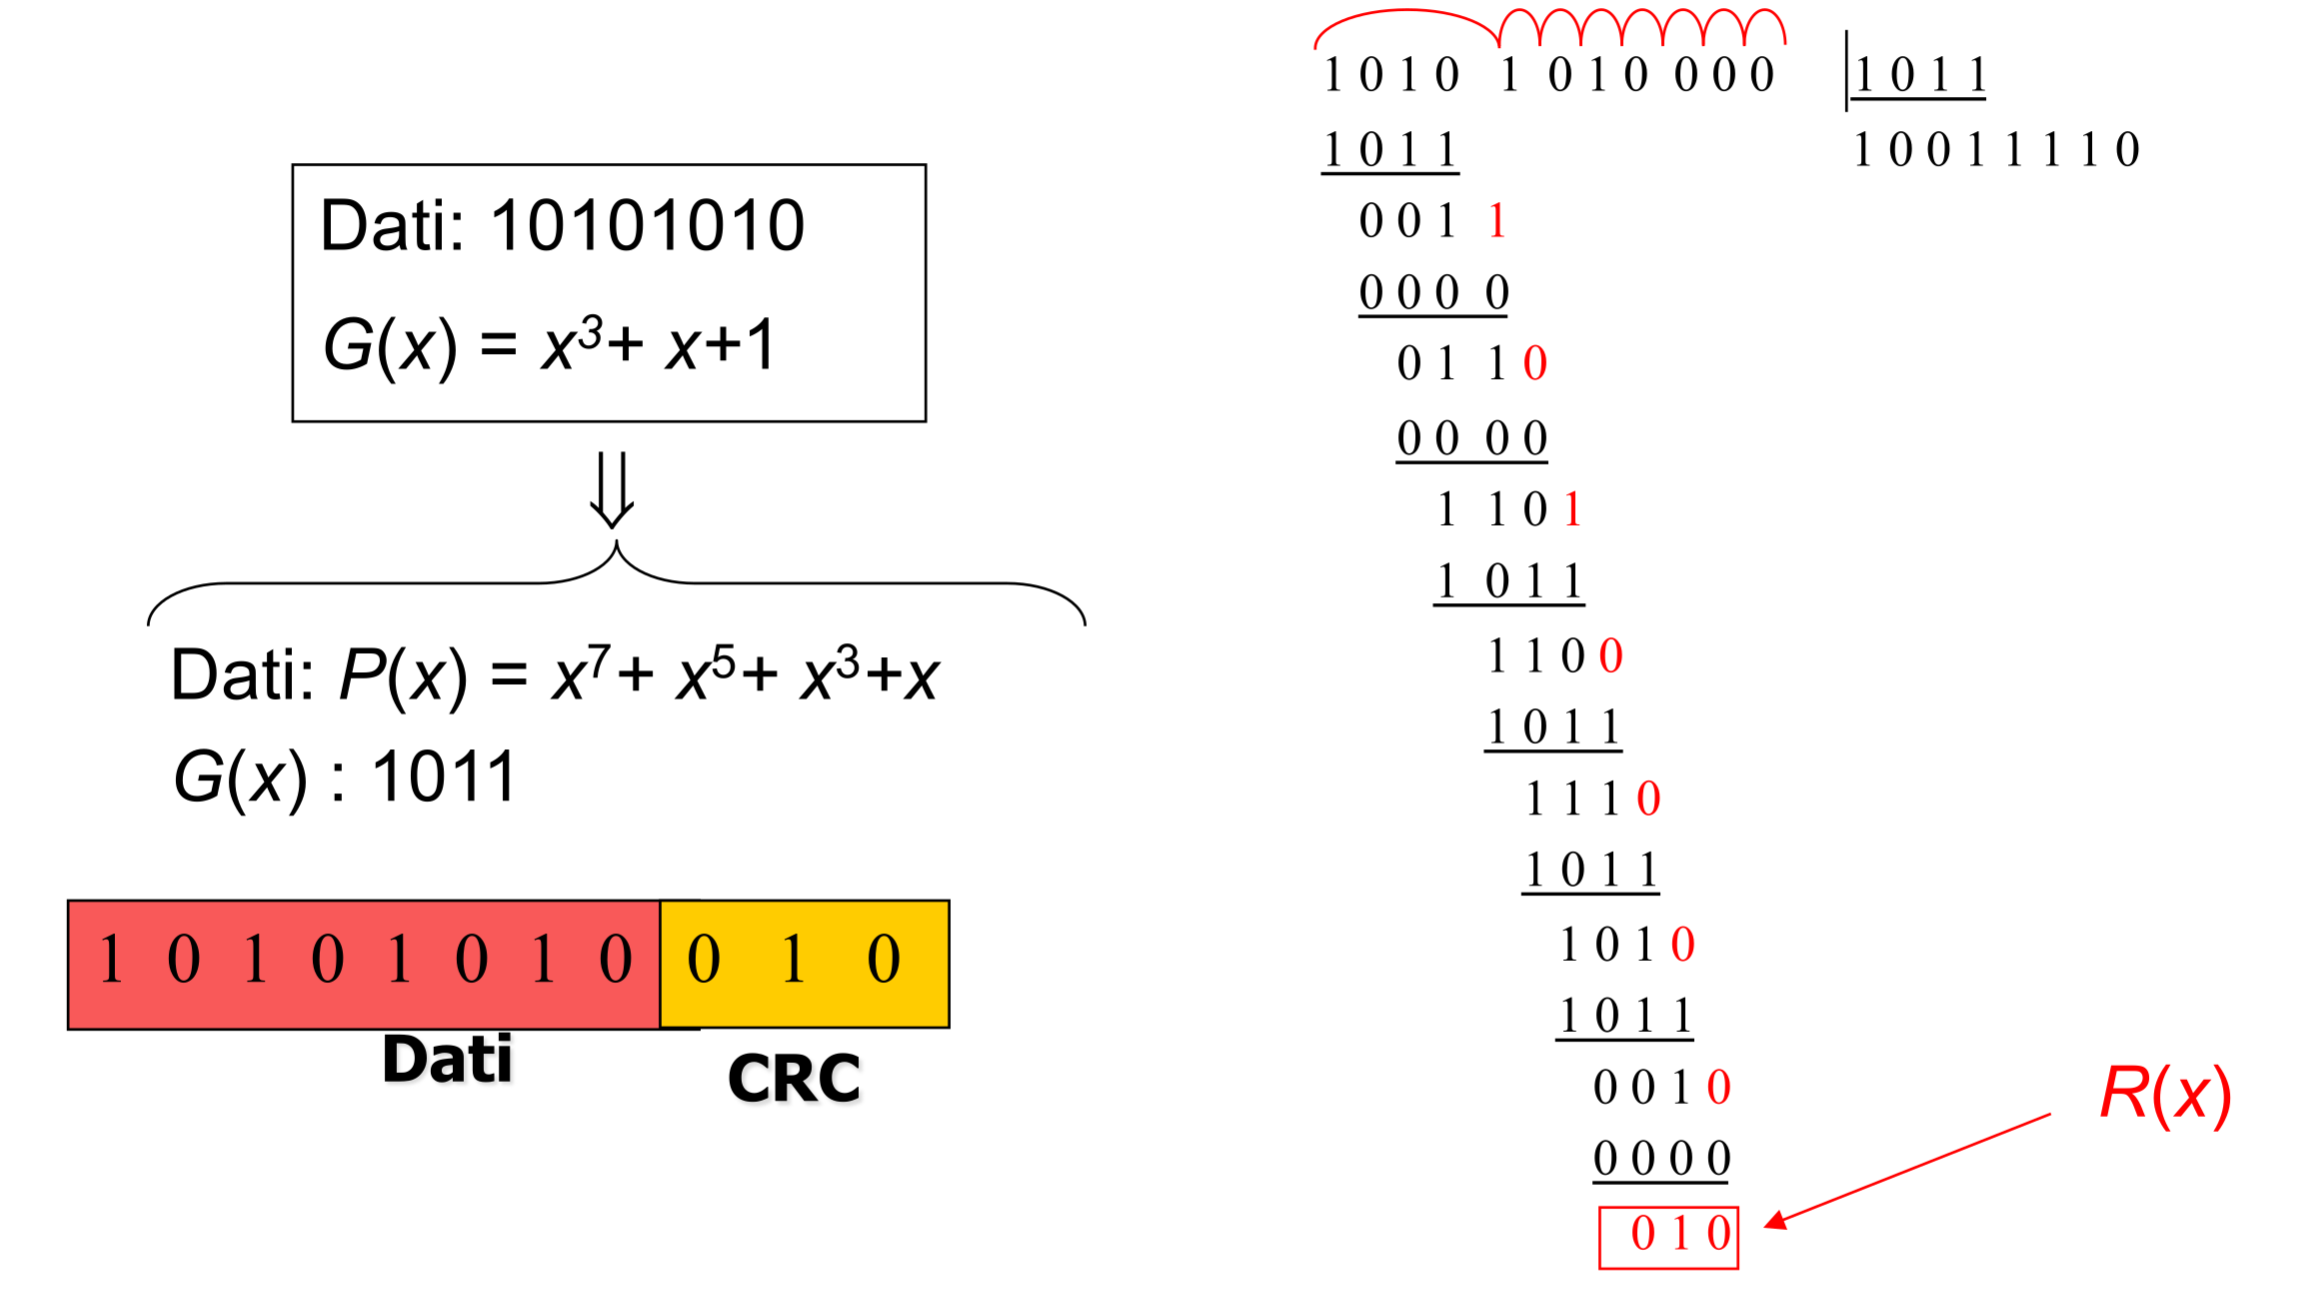
\includegraphics[width=0.8\textwidth]{images/esempiocrc.png}
        \caption{Esempio di calcolo CRC}
        \label{fig:esempio-crc}
    \end{figure}

    \subsection{Protocollo point to point (PPP)}

    \begin{figure}[htbp]
        \centering
        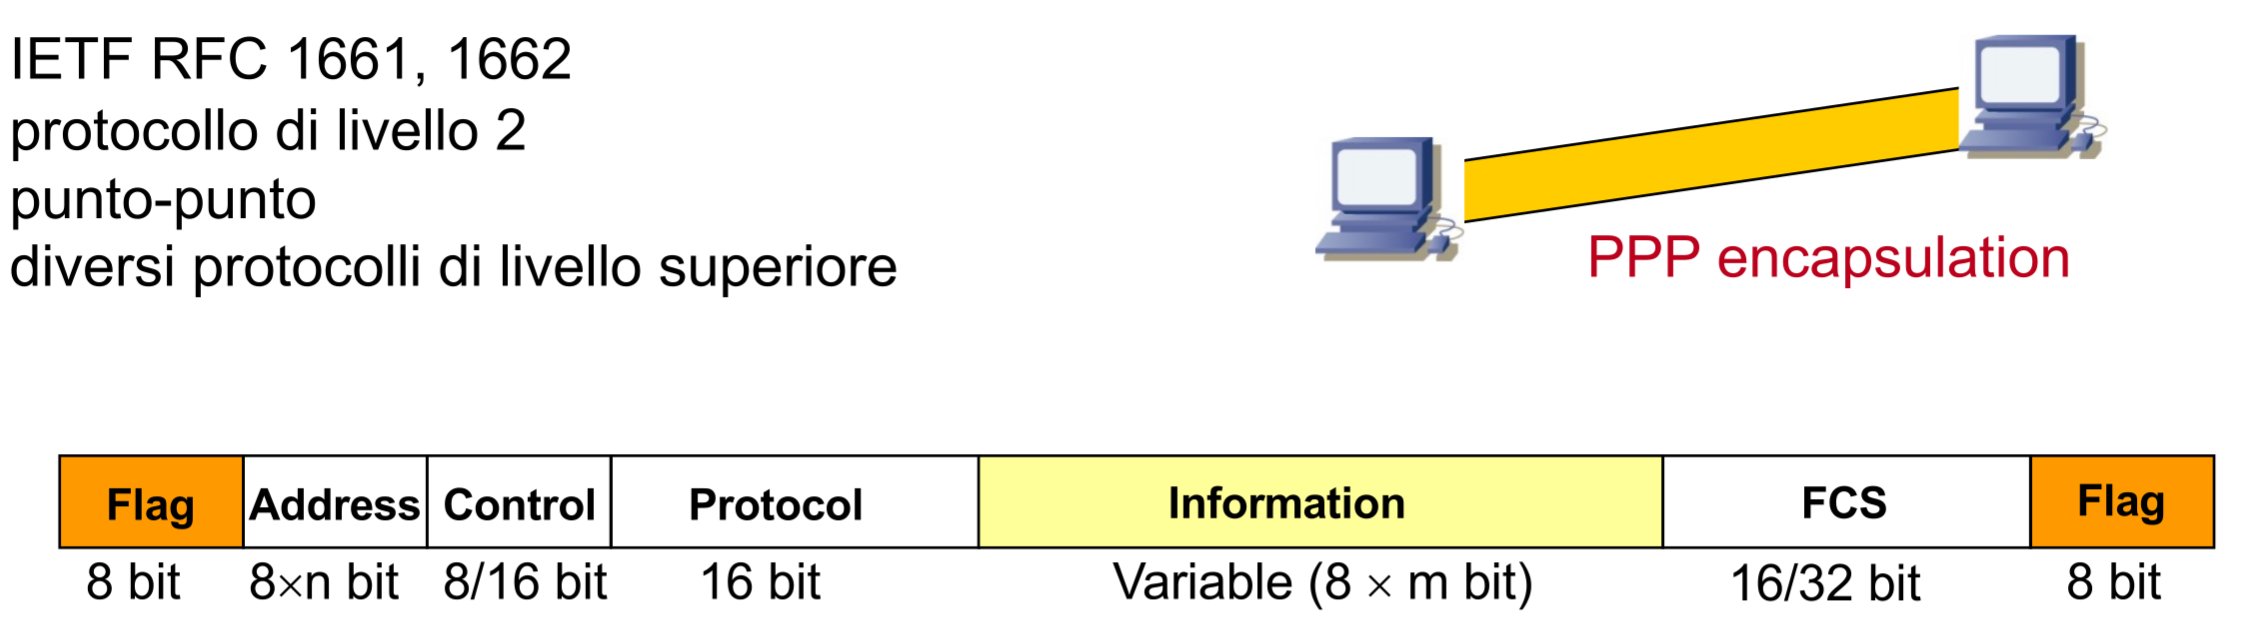
\includegraphics[width=0.85\textwidth]{images/pointtopoint.png}
        \caption{Protocollo Point to Point}
        \label{fig:point-to-point}
    \end{figure}

Il protocollo Point to Point è comunemente usato nello stabilire connessioni dirette tra due nodi.

Il frame è quasi identico a quello del HDLC, ha un campo aggiuntivo, quello protocol: specifica il protocollo di livello 3 che stiamo trasportando.

\paragraph{Network bit order - Big Endian e Little Endian}
A differenza dello standard HDLC, big-endian, il protocollo PPP non è endianness specifico.

L'ordine dei byte (conosciuto anche come big-endian, little-endian o middle-endian a seconda dei metodi differenti), in informatica, indica modalità differenti usate dai calcolatori per immagazzinare all'interno della memoria dati di dimensione superiore al byte;dipende essenzialmente dall'architettura hardware usata.

"I termini big-endian e little-endian derivano dai nomi di due popolazioni che abitavano nelle favolose isole di Lilliput e Blefuscu nel romanzo I viaggi di Gulliver di Jonathan Swift. Queste erano entrate in rivalità per il modo in cui aprivano le uova - rompendo la punta o il fondo: a Lilliput, per editto dell'imperatore il cui figlio una volta si tagliò aprendo un uovo dall'estremità più grande, fu ordinato di aprire le uova dall'estremità più piccola (little endians); a Blefuscu si rifugiarono gli oppositori che volevano conservare la tradizione di rompere le uova dall'estremità più grande (big endians). A causa di questa differenza e della sua legittimazione imperiale era scoppiata tra le due isole una guerra sanguinosa."

\begin{figure}[htbp]
    \centering
    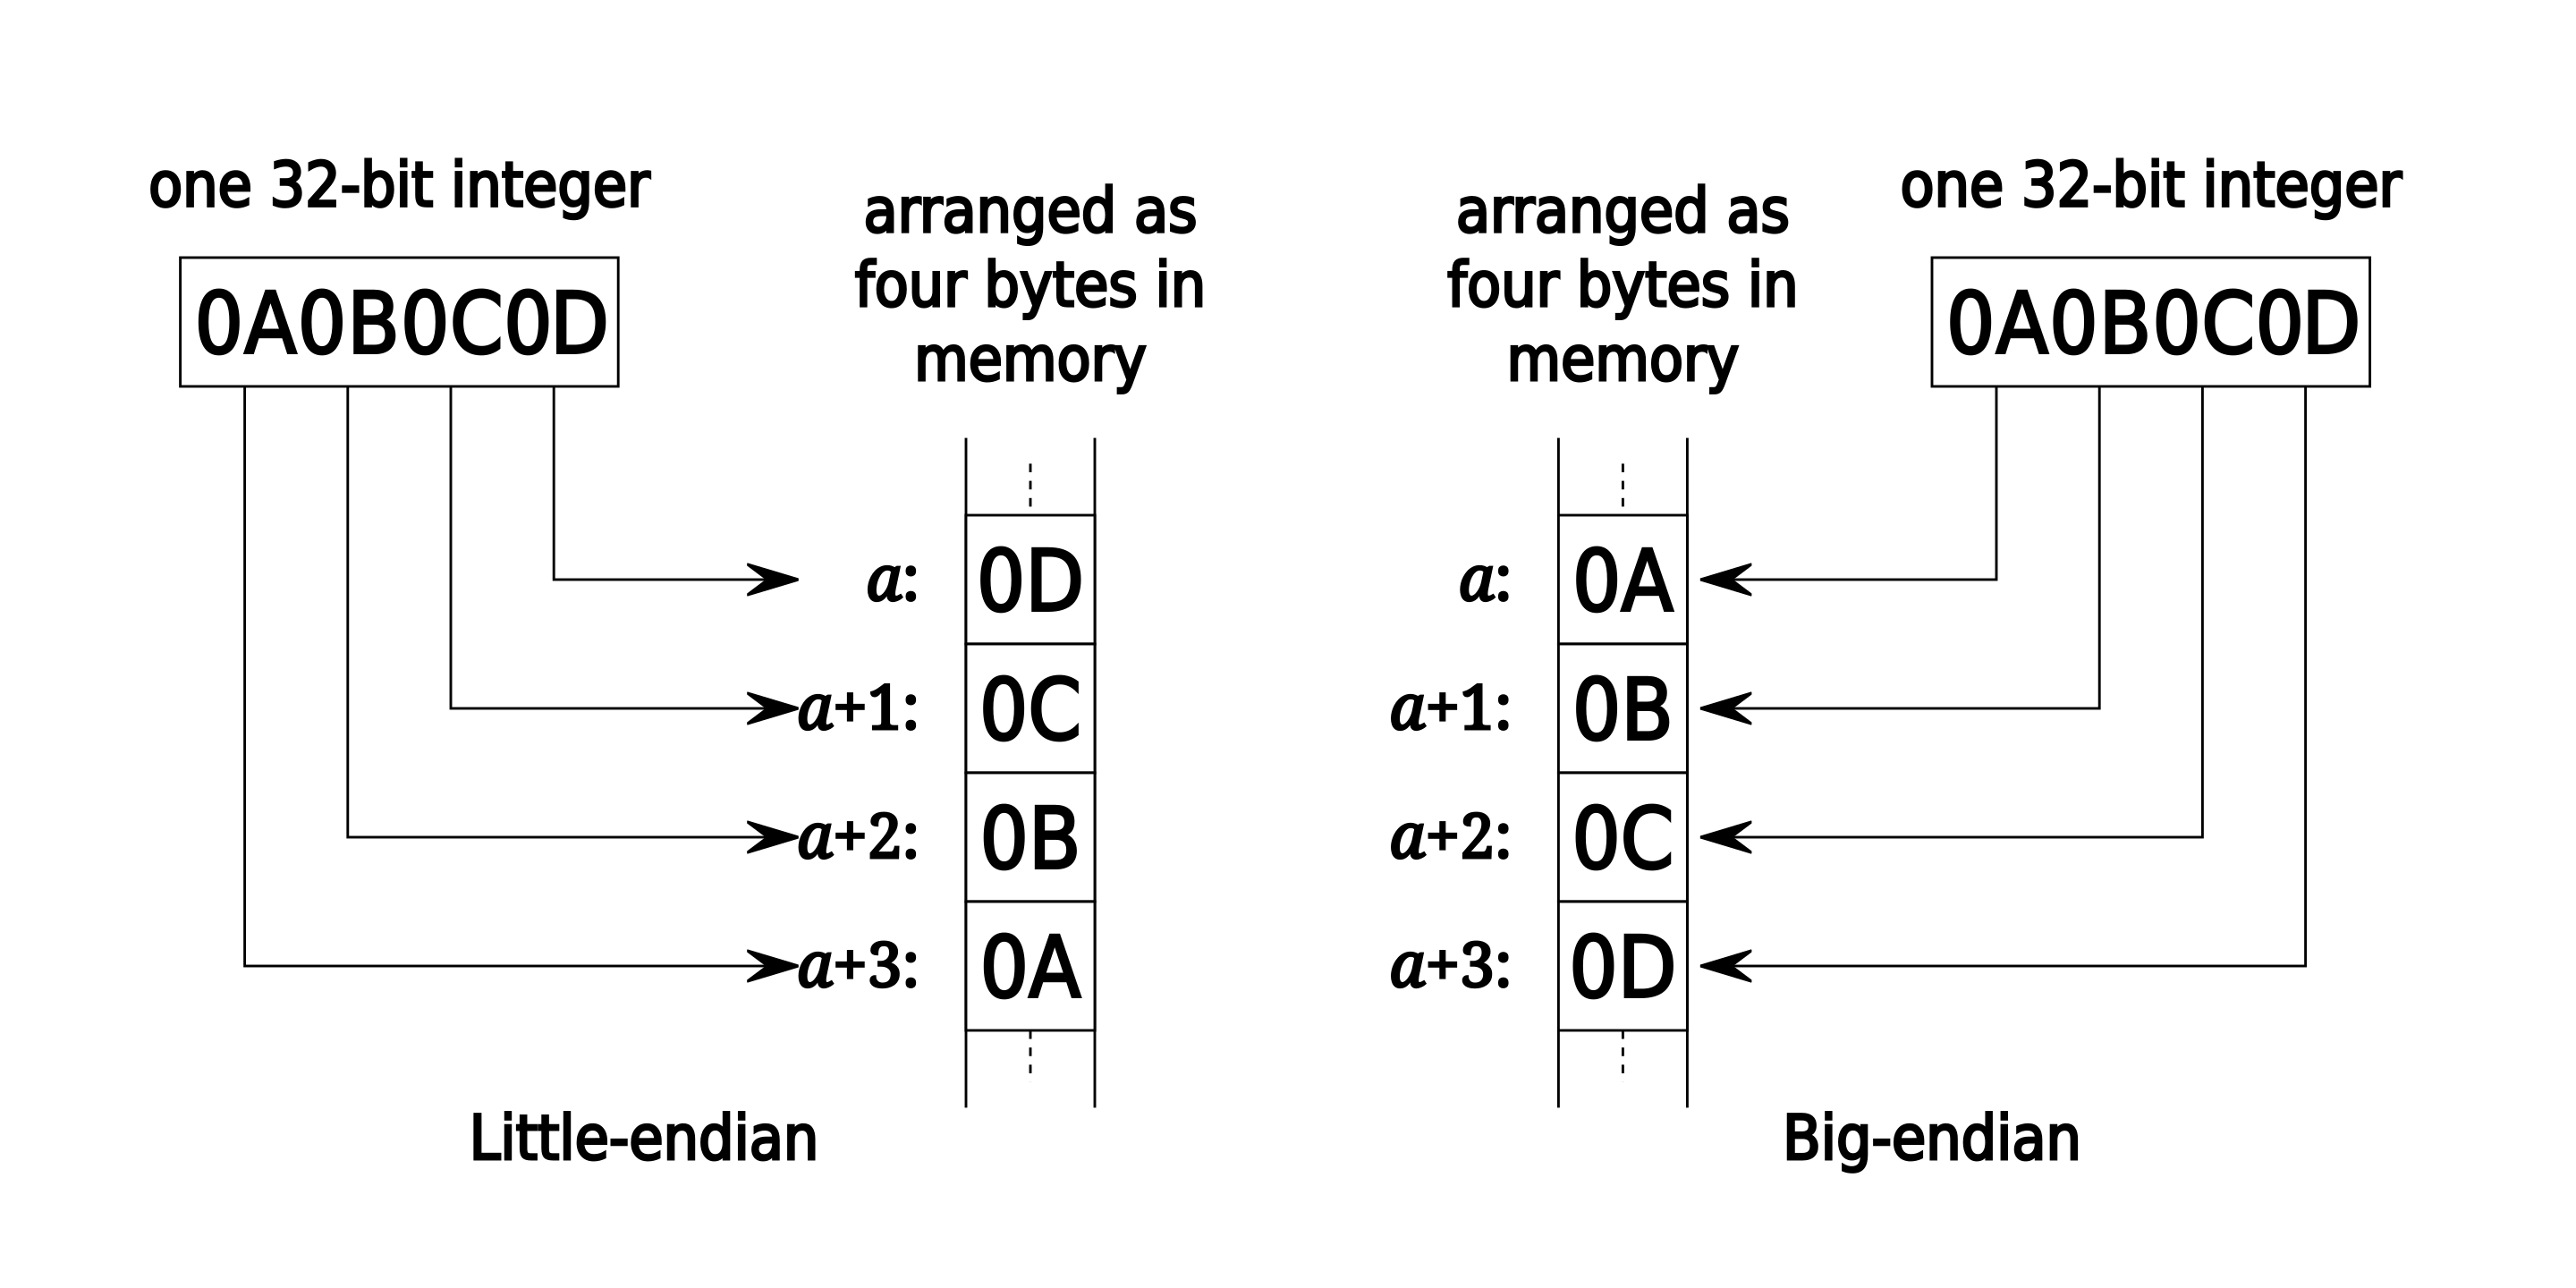
\includegraphics[width=0.8\textwidth]{images/endian.png}
    \caption{Big Endian e Little Endian}
    \label{fig:endian}
\end{figure}
\newpage

    \subsubsection{Byte stuffing}


    Anche qui, vista la struttura del pacchetto molto simile a quella del frame HDLC, c'è il rischio di confondere il dato informativo con un flag; perciò si attua il byte stuffing.

    \paragraph{Sequenza di flag 0x7d}

    Se si vuole evitare la sequenza 0x7e (01111110), si antepone la sequenza di controllo 0x7d (01111101); al posto della sequenza 0x7e inseriamo la sua versione in XOR con la sequenza 0x20 (00100000).
    
    A quel punto avremo individuato la sequenza "pericolosa" all'interno del frame, ossia 0x7e, avremo un identificativo, 0x7d, che ci dice dov'è situata nel frame e la sostituiremo con il suo valore in XOR con 0x20.
     
    Quindi quando all'interno del frame leggo il byte 0x7d, il nuovo flag che indica che c'è stato byte stuffing, non leggiamo 0x7d ma il byte successivo, quello calcolato tramite il 0x7e XOR 0x20.

    In ricezione se applico nuovamente XOR 0x20 al byte precedentemente modificato con lo XOR, allora otterrò nuovamente il byte iniziale, 0x7e.
    
    
    
    \begin{figure}[htbp]
        \centering
        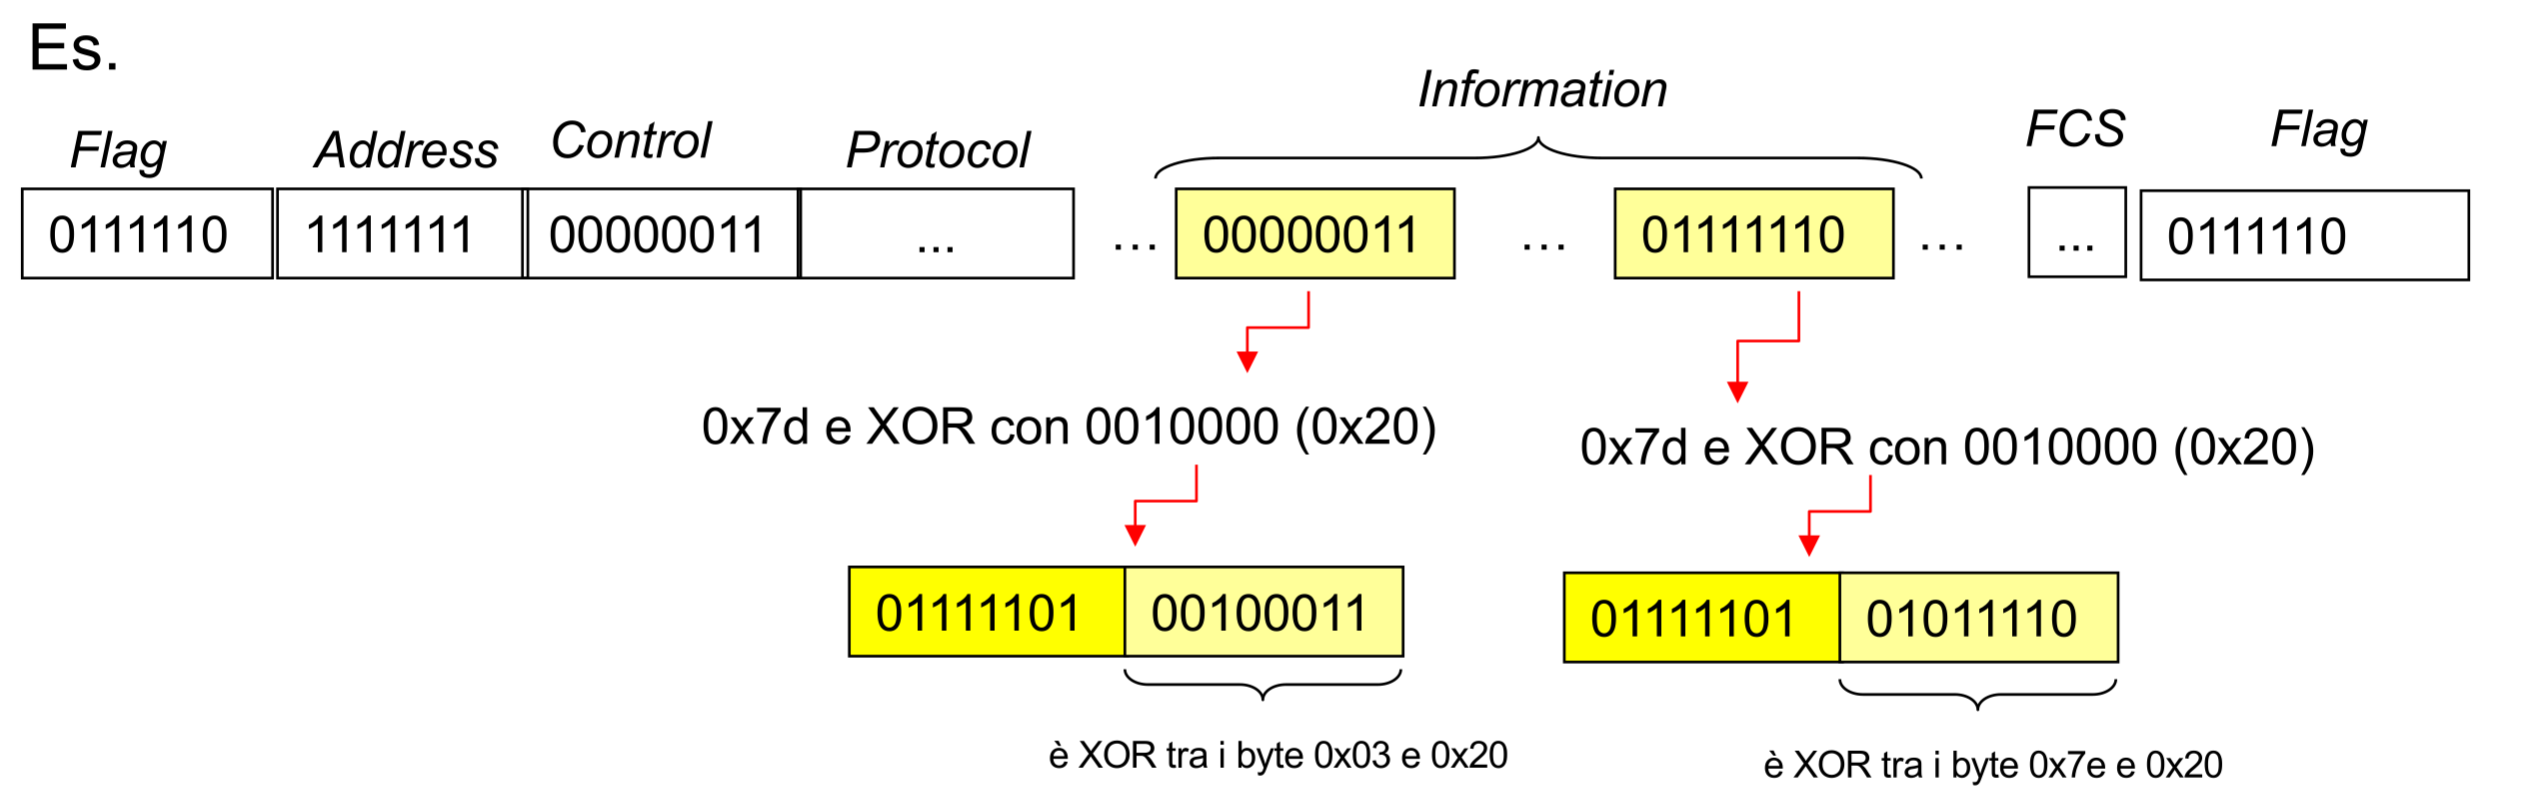
\includegraphics[width=1\textwidth]{images/bytestuffing.png}
        \caption{Esempio di byte stuffing}
        \label{fig:byte-stuffing}
    \end{figure}

    Nel caso in cui incappiamo con una "falsa" sequenza di flag del byte stuffing, ossia 0x7d, la trasmettermo come 0x7d, 0x5d.
     
    \subsubsection{Struttura PPP}

    Il PPP utilizza due protocolli per la gestione del collegamento tra nodi:
    
    \begin{figure}[htbp]
        \centering
        \begin{minipage}{0.45\textwidth}
            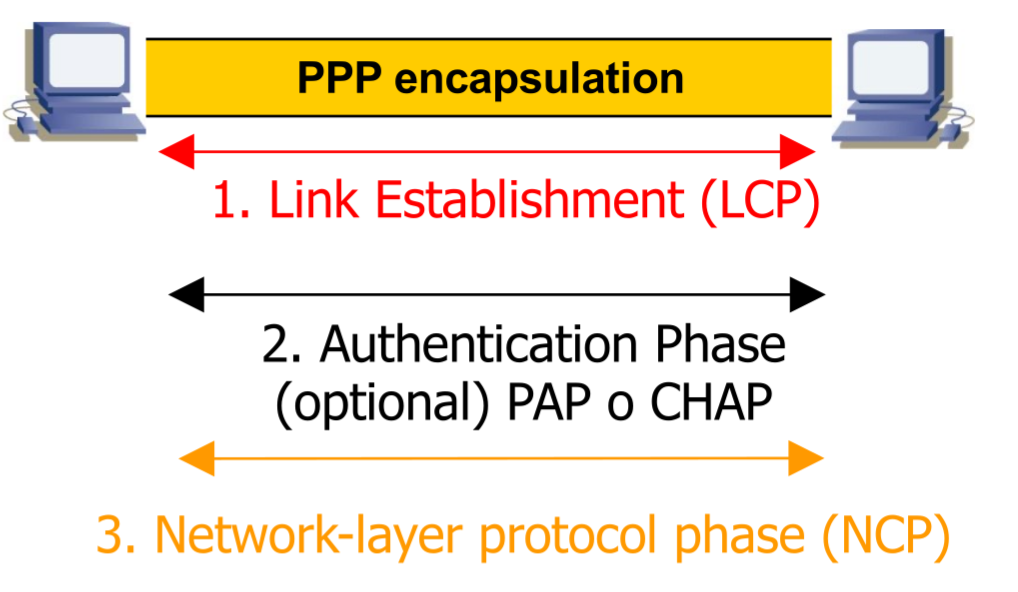
\includegraphics[width=\linewidth]{images/pppencapsulation.png}
            \caption{Encapsulation PPP}
            \label{fig:ppp-encapsulation}
        \end{minipage}%
        \hfill
        \begin{minipage}{0.5\textwidth}
            \begin{itemize}
                \item LCP(Link Control Protocol): grazie al quale si apre la connessione, si ha la verifica della qualità del collegamento e rende possibile l'autenticazione(PAP o CHAP)
                \item NCP(Network Control Protocol): con cui è possible scegliere e configurare uno o più protocolli di rete(es. IP)
            \end{itemize} 

        \end{minipage}
    \end{figure}
\newpage
    \subsubsection{Autenticazioni}
    \begin{figure}[htbp]
        \centering
        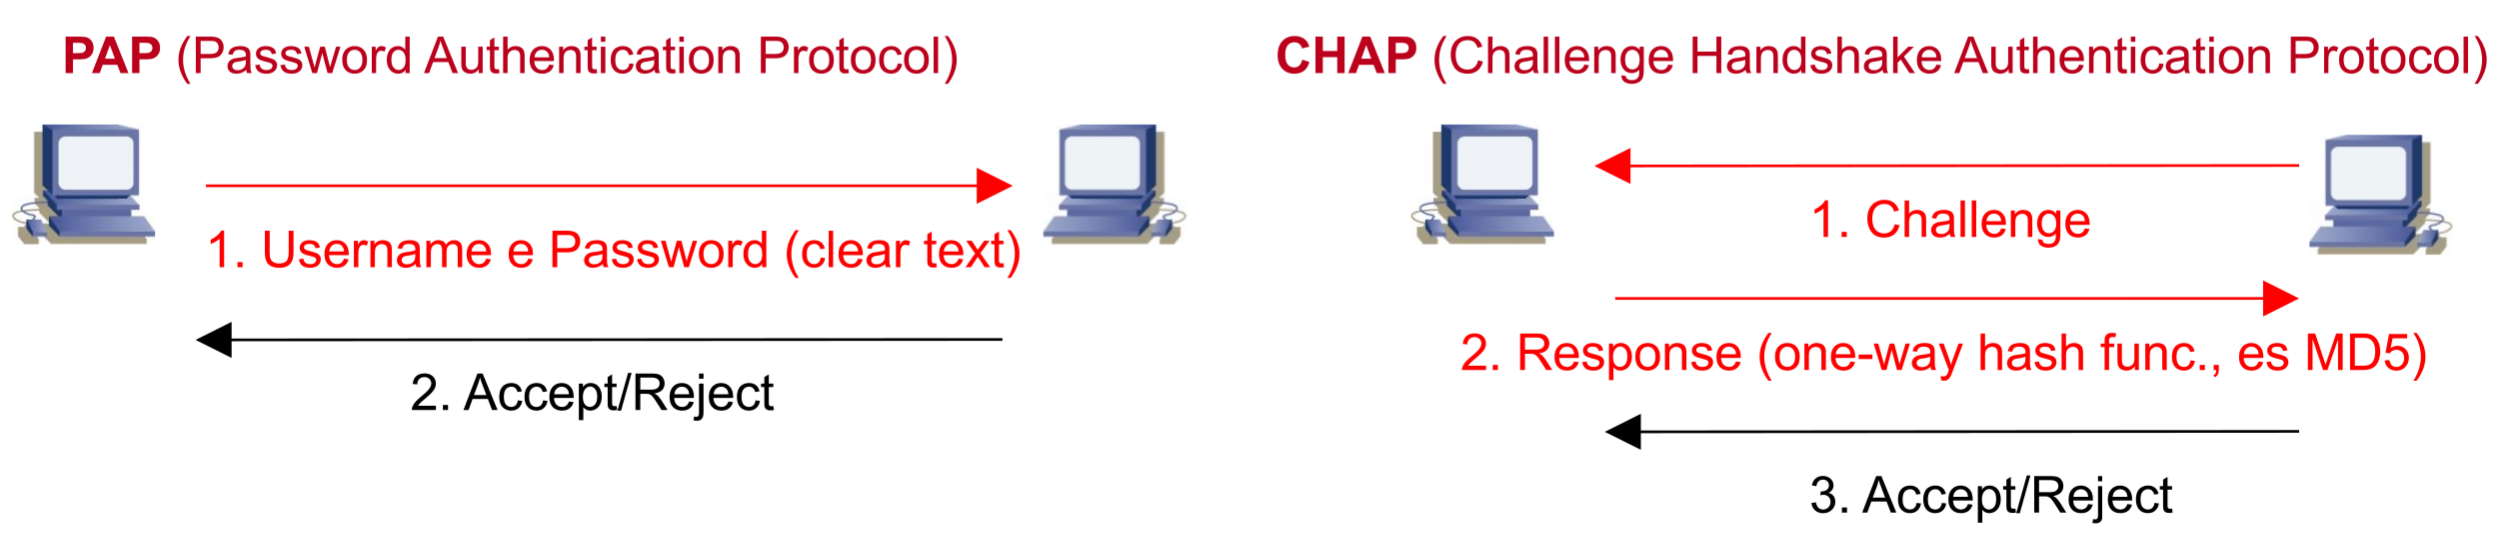
\includegraphics[width=1\textwidth]{images/autenticazionecapchap.png}
        \caption{Autenticazione PAP e CHAP}
        \label{fig:autenticazione-pap-chap}
    \end{figure}
    \paragraph{Autenticazione PAP} 
    Password Authentication Protocol (PAP) invia username e password in chiaro. È semplice ma poco sicuro, poiché le credenziali possono essere intercettate(password e username sono solitamente criptate).

    \paragraph{Autenticazione CHAP} 
    Challenge Handshake Authentication Protocol (CHAP) utilizza un meccanismo di challenge-response con hash per autenticare in modo più sicuro, evitando di trasmettere la password in chiaro.


\section{Protocolli di accesso}
A livello due viene svolto un ruolo importante dai protocolli di accesso, che possono essere di due tipologie:
\begin{itemize}
    \item Accesso ordinato:
    \begin{itemize}
        \item Ogni nodo ha un turno prestabilito per trasmettere, evitando collisioni.
        \item Utilizzato in sistemi come il polling o il token passing.
        \item Garantisce un utilizzo equo del canale, ma può introdurre ritardi se un nodo non ha dati da trasmettere.
    \end{itemize}
    \item Accesso casuale:
    \begin{itemize}
        \item senza rilevazione del canale:
        \begin{itemize}
            \item I nodi trasmettono senza verificare se il canale è libero.
            \item Può portare a collisioni frequenti, come nel protocollo ALOHA puro.
        \end{itemize}
        \item con rilevazione del canale:
        \begin{itemize}
            \item senza rivelazione di collisioni:
            \begin{itemize}
                \item I nodi verificano se il canale è libero prima di trasmettere.
                \item Non rilevano collisioni, quindi i dati persi devono essere ritrasmessi dopo un timeout.
                \item Esempio: Carrier Sense Multiple Access (CSMA).
            \end{itemize}
            \item con rilevazione di collisioni:
            \begin{itemize}
                \item I nodi verificano se il canale è libero e rilevano eventuali collisioni durante la trasm.
                \item In caso di collisione, interrompono la trasm. e ritentano dopo un intervallo casuale.
                \item Esempio: CSMA/CD (utilizzato in Ethernet).
            \end{itemize}
        \end{itemize}
    \end{itemize}
\end{itemize}
\newpage

\subsection{Troughput di rete}
\subsubsection{Calcolo del Troughput}

\subsection{Protocollo ALOHA puro}
ALOHA è un protocollo di accesso multiplo casuale senza rilevazione del canale, 

\subsubsection{Calcolo del Troughput di ALOHA puro}

\subsubsection{Prestazioni ALOHA puro}

\subsection{Protocollo ALOHA slotted}
\subsubsection{Prestazioni ALOHA slotted}

\subsection{Protocolli Carrier Sense Multiple Access - CSMA}
\subsubsection{CSMA/CD}


\subsubsection{CSMA/CA}
